\documentclass[11pt]{article}
\usepackage{tikz}
\usepackage{algorithm}
\usepackage{algpseudocode}
\usepackage{amsmath}
\begin{document}
\title{DGSAND: A Discontinuous Galerkin Sand box }
\author{Jay Sitaraman}
\maketitle
\section{Background}
It has been on my wish list for a long time to write a simple Discontinuous Galerkin code that can be used
for testing efficiency and algorithm modifications towards creating a more efficient GPU centric implementation.
Finally, I have been able to take a few weeks away from the routine work and put some focussed time on reading
papers and writing a code that actually works at least for a simple problem. There are several other open
source DG codes produced by many different groups available on the internet. Therefore, it is natural to
wonder whetherthere is a need for having yet another code. I don't have a good answer for this other
than saying that doing something by myself is the only way I know to learn well enough to be able
to explain the same to others. I am grateful to Mike Brazell and Hari Sitaraman for sharing their more
sophisticated discontinuous galerkin codes for me to take inspiration from. I am also grateful to Steve Tran
and Beatrice Roget for their 1-D codes that provided the mathematical basis for the implementation here.
I have tried to simplify the notations in the mathematical description below as much as possible to make it
accessible to engineers. In general, I have found most of the finite element method papers rely more than
their necessary share on mathematical notation for brevity and appearence of eruditeness.
This does tend to frustrate competent engineers who could otherwise have contributed meaningfully to a project. 

\section{Software}
This code is written in pure C with the intention that it can be easily ported to CUDA/HIP as and when it is
possible to do so without any major changes to underlying source. I have also tried to minimize the number
of if conditions and possible race scenarios by arranging the loops in fashion slightly different
from standard finite volume/finite element codes. There is definitely still a very large room for optimization.
I have also stayed away from C++ and usage of any templating
because of my own aversion to their over-use in modern codes and also concerns on their efficiency
(both of these concerns may be misplaced). Instead, I have opted for a straight arrays that can be indexed in to
for picking out the appropriate geometric and field values per element. All filling is done in standard C order
order as field values for each degree of freedom for every field for every element. Finally I have also tried
(at least for now) to not have any dependencies and stick to as simple a compilation system as
possible to build the code. 

\section{Mathematical Framework}
The conservation law for first order hyperbolic systems are given by :
\begin{equation}
  \frac{\partial Q}{\partial t} + \nabla \cdot F(Q) = 0
  \label{eq1}
\end{equation}
where $Q$ is the conserved variable and $F(Q)$ is the flux of this variable~\cite{wikipedia}. In a
Discontinuous Galerkin Finite Element Method, implemented in a semi-discrete form (i.e finite elements in space
only), the space is split into $N_e$ non-overlapping elements.
Each element is then equipped with a basis set (which are almost always polynomials) that
approximate the variation of a field within that element. The coefficients of these polynomials are the
unknowns that need to be solved using the chosen numerical method. The finite element method, in this sense
is a glorified curve-fitting approach, where the method used to reduce the constraint that the unknowns
must satisfy the partial differential equation and its boundary condition into a set of algebraic equations
usually defines the type of the method. In a ``Discontinuous'' approach, all of the basis set of an element is
constrained to have identically zero values outside of that element. This stands in contrast to a
more well known ``continuous'' approach where the basis associated with a degree of freedom will have
non-zero values on every element that shares it. Following notations used by
Atkins~\cite{atkins}, the basis set is represented as:
\begin{equation}
  B \equiv \{b_k, 1 \leq k \leq N(e,p,d)\}
\end{equation}
Each basis $b_k$ to a particular order is a polynomial of order $p$ of the barycentric
coordinates within the reference element, e.g. in 2-D it would be a polynomial composed of
monomials from the set $\{1,x,y,x^2,xy,y^2,x^2y,xy^2,x^3..\}$ etc where $\{x,y\}$ represent
location within an element. $N(e,p,d)$ represents
the number of linearly independent basis functions required to fully represent the spatial variation
upto polynomial order $p$ for element type $e$ in dimensions $d$.  In this work, a
hierarchical basis is chosen for ease of implementation. The chosen basis for
triangles (only ones implemented at this time) are taken from MontJoie user manual
~\cite{montjoie}. Once the basis set is chosen, the field at any location within an
element can be approximated (to a given order $p$) as  as a summation as shown below
\begin{equation}
  Q_i(u) = \sum_{k=1}^{k=N_i} {q_k}_i {b_k}_i(u)\
\end{equation}
Here $u$ is the coordinate vector, e.g. $u=\{x,y\}$ in 2D and
$u=\{x,y,z\}$ in 3D etc. The subscript $i$ represents a given element $i$. The entire vector field
$Q$ is the union of the approximate solutions that are valid within each element. To reiterate,
the basis functions ${b_k}_i$ are zero everywhere outside element $i$. So one can express
the field Q approximately as
\begin{equation}
  Q_f=\sum_{i=1}^{i=N_e} \sum_{k=1}^{k=N_i} {{(q_k}_f)}_i {b_k}_i \hspace{0.5in} f\in[1,nfields]
  \label{eq2}
\end{equation}
The total number of unknowns (${({q_k}_f)}_i$) are $ndof=nfields*\sum_{i=1}^{i=N_e} N_i$, where nfields is the number of
conservation equations at a given spatio-temporal location, e.g. for 2-D Navier-Stokes it will be 4
consiting of conservation of mass (1 eqn), conservation of momentum (2 eqns) and conservation of
energy (1 eqn). Substituting in Eq.~\ref{eq2} in Eq.~\ref{eq1} and omitting the subscripts $i$ and $f$
for clarity one obtains
\begin{equation}
  \frac{\partial (\sum \sum{q_k b_k })}{\partial t} + \nabla \cdot F(\sum \sum q_k b_k) = 0
  \label{eq3}
\end{equation}
If the flux $F$ is differentiable across element interfaces one could use Eq.~\ref{eq3} directly to
obtain $ndof$ equations for the unknown vector ${({q_k}_f)}_i$. Weaker or integral formulations are more general
since they do not require differentiability or even continuity across element interfaces. In general, weaker
formulations are constructed by multiplying Eq.~\ref{eq3} by a test function and integrating across the entire
domain (Galerkin formulation). One of the constraint for the test functions are that they  have to
maintain linear independence to create a well posed system of algebraic equations. A convenient choice of the
test functions are the basis function themselves which leads to the following weak integral form. 
\begin{equation}
  \int_{\Omega} b_j\left[\frac{\partial (\sum \sum{q_k b_k })}{\partial t} + \nabla \cdot F(\sum \sum q_k b_k)\right] d \Omega=0
\end{equation}
Where $\Omega$ represents the entire space where the conservation law is to be enforced. Noting again that ${b_j}_i$ are ${b_k}_i$ are non-zero only within an element $i$, this space of integration can be reduced to be just within each
element for the basis that are associated with that element. 
\begin{equation}
  \int_{\Omega_i} {b_j}_i\left[\frac{\partial (\sum{{({q_k}_f)}_i} {b_k}_i)} {\partial t} + \nabla \cdot F(Q_i)_f\right] d \Omega_i=0
  \label{eq4}
\end{equation}
Equation~\ref{eq4} represents one of the semi-discrete equations in element $i$ assocated with
basis ${b_j}_i$. Note that $(Q_i)_f = \sum \sum (q_k)_f b_k$, where f is the index of the field and $F(Q_i)_f$ is the $f^{th}$ row
of the flux of $Q_i$. There are $N$ such equations per field within each element. Combining all of the equations
for element $i$ for a given field $f$ and dropping the subscript $i$ for basis and the unknowns yields $N$ equations
that can be written as:
\begin{equation}
  \left[\int_{\Omega_i} {b_j} {b_k} d\Omega_i\right]\frac{\partial ({q_k})_f}{\partial t} + \int_{\Omega_i} {b_j} \nabla \cdot F(Q)_f d \Omega_i = 0, \hspace{0.1in} j,k \in [1,N] 
  \label{eq5}
\end{equation}
Note that $b_j$ are $b_k$ are pure spatial functions and hence can be taken outside of the time derivative. The
unknowns (polynomial coefficients) are functions of time and the time derivative operator is applied to them. The
first term in Eq.~\ref{eq5}, $[..]$, is termed the mass matrix in finite element parlance since it scales a
velocity derivative akin to a mass-spring-damper equation common in structural dynamics. Each term of the
$N \times N$ mass matrix is the integration of the product of each pair of basis functions (including itself)
within that element. Considering the second term, of equation ~\ref{eq5}, one can observe it is the product
of scalar with the divergence of a vector. The product rule of divergence is
\begin{equation}
  \nabla \cdot (b F) = b\nabla .F + \nabla b.F
  \label{eq6}
\end{equation}
This is nothing but the generalization of the product rule of derivative in single dimension, which is simply $\frac{\partial (uv)}{\partial x} = u \frac{\partial v}{\partial x} + \frac{\partial u}{\partial x} v$.
From Eq.~\ref{eq6}, \newline $b \nabla.F = -\nabla b.F + \nabla \cdot (b F)$, substituting in Eq.~\ref{eq5} yields:
\begin{equation}
  \left[\int_{\Omega_i} {b_j} {b_k} d\Omega_i\right]\frac{\partial {(q_k)_f}}{\partial t} - \int_{\Omega_i} \nabla b_j  
\cdot F(Q)_f d \Omega_i + \int_{\Omega_i} \nabla \cdot (b_j F(Q)_f) d \Omega_i = 0
  \label{eq7}
\end{equation}
Where $Q_i^f$ is the approximation within the element $i$ for field $f$ given by $\sum {q^f_k}_i {b_k}_i$. Using
Gauss-divergence theorem the third term, which is a volume integral that can be expressed as a surface integral
over the boundary surface of the element ($\partial \Omega_i$), one obtains:
\begin{equation}
  \left[\int_{\Omega_i} {b_j} {b_k} d\Omega_i\right]\frac{\partial {(q_k)_f}}{\partial t} - \int_{\Omega_i} \nabla b_j
\cdot F(Q)_f d \Omega_i + \int_{\partial\Omega_i} b_j F(Q)_f \cdot \vec{ds}  = 0
\label{eq8}
\end{equation}
At this point we have to develop methods for evaluating the integrals above within and
around each element to a sufficient accuracy. 

\subsection{Coordinate Transformation}
Every element can be mapped on to a reference element as shown below. Elements in physical
space may have curved boundaries, but the reference elements are unit dimensional with
planar faces. An example for a triangle is shown below  \newline
\begin{tikzpicture}
  \draw[->] (-0.5,-0.5) -- (1.0,-0.5)  ;
  \draw[->] (-0.5,-0.5) -- (-0.5,1.0)  ;
  \draw (1.0,-0.75) node {x};
  \draw (-0.75,1.0) node {y};
  \draw (0,0) .. controls (1,0.2) .. (2,0) -- (1.0,1.7) -- cycle;
  \draw [->] (3,0.5) -- (6,0.5) ;
  \draw (7,0) -- (9,0) -- (7,2)--cycle;
  \draw [->] (7,0) -- (10,0);
  \draw [->] (7,0) -- (7,3);
  \draw (10,-0.25) node {r};
  \draw (6.75,3) node {s};
  \draw (6.5,-0.25) node{(0,0)};
  \draw (9.0,-0.25) node{(1,0)};
  \draw (6.5,2.0) node{(0,1)};
\end{tikzpicture}
\newline
The transformation between $(x,y,z)\in \Omega$ physical coordinates in 3D and the
$(r,s,t)\in \Lambda$ coordinates within the reference element can be written as:
\begin{equation}
\begin{bmatrix}
  \frac{\partial x}{\partial r} & \frac{\partial x}{\partial s} & \frac{\partial x}{\partial t}\\
  \frac{\partial y}{\partial r} & \frac{\partial y}{\partial s} & \frac{\partial y}{\partial t}\\
  \frac{\partial z}{\partial r} & \frac{\partial z}{\partial s} & \frac{\partial z}{dt}
\end{bmatrix}
\begin{bmatrix}
  dr\\
  ds\\
  dt\\
\end{bmatrix}
=
\begin{bmatrix}
  dx \\
  dy \\
  dz \\
\end{bmatrix}
\end{equation}
Where
\begin{equation}
  J=\frac{\partial(x,y,z)}{\partial(r,s,t)} =
  \begin{bmatrix}
  \frac{\partial x}{\partial r} & \frac{\partial x}{\partial s} & \frac{\partial x}{\partial t}\\
  \frac{\partial y}{\partial r} & \frac{\partial y}{\partial s} & \frac{\partial y}{\partial t}\\
  \frac{\partial z}{\partial r} & \frac{\partial z}{\partial s} & \frac{\partial z}{dt}
\end{bmatrix}
\end{equation}
is the Jacobian of transformation. Similarly in 2D the transformation will be:
\begin{equation}
  J=\frac{\partial(x,y)}{\partial(r,s)} =
  \begin{bmatrix}
  \frac{\partial x}{\partial r} & \frac{\partial x}{\partial s}  \\
  \frac{\partial y}{\partial r} & \frac{\partial y}{\partial s}  \\
\end{bmatrix}
\end{equation}
The integrals in Eq.~\ref{eq8} has both volume integral and surface integral terms
and these need to be transformed to the reference element to perform the integration.
\subsubsection{Transformation of Volume integrals}
Considering 2-D, the differential volume (really area in 2D)
for integration is often denoted in literature as
$d\Omega = dxdy$, however it is actually $\vert dx \hat{e_x} \times dy\hat{e_y} \vert$.
In Cartesian coordinate system,  the unit vectors $\hat{e_x}$ and $\hat{e_y}$
are orthogonal to each other and hence the differential area reduces to simply $dxdy$.
The vector $dx \hat{e_x}$ can be expressed as
$dx \hat{e_x} = (\frac{\partial x}{\partial r} dr)\hat{e_r} +  (\frac{\partial x}{\partial s} ds) \hat{e_s}$ using
vectors $\hat{e_r}$ and $\hat{e_s}$ of the the reference coordinate system. Note that
$\hat{e_r}$ and $\hat{e_s}$ are still in the physical coordinate system and not necessarily
orthogonal to each other.  However, $\hat{e_r} \times \hat{e_s}$ always points in the same
direction. Using these ideas, we can expand
\begin{eqnarray}
  \vert dx \times dy \vert = \left \vert \left((\frac{\partial x}{\partial r}dr)\hat{e_r}+(\frac{\partial x}{\partial s}ds)\hat{e_s}\right) \times \left((\frac{\partial y}{\partial r}dr)\hat{e_r}+(\frac{\partial y}{\partial s}ds)\hat{e_s} \right )\right \vert \\ = \left \vert \frac{\partial x}{\partial r}\frac{\partial y}{\partial s} - \frac{\partial y}{\partial r}\frac{\partial x}{\partial s} \right \vert drds\\
  = |J|drds
\end{eqnarray}
Where $|J|$ is the determinant of the Jacobian of transformation.
In similar vain, the differential volume in 3D is given by the triple product 
$dx\hat{e_x}.(dy\hat{e_y} \times dz\hat{e_z})$ in physical coordinate space,
which transforms to $|J|drdsdt$ within the reference element.

\subsubsection{Transformation of Surface integral}
The integrals of type $\int_{d\Omega} (..).\vec{\partial s}$ is the same as $\int_{d\Omega} (..) \cdot \hat{n} |ds|$, where $\hat{n}$ is the unit normal on the element surface (this would vary for
elements with curved boundaries). Consider the prismatic reference element below:
\newline
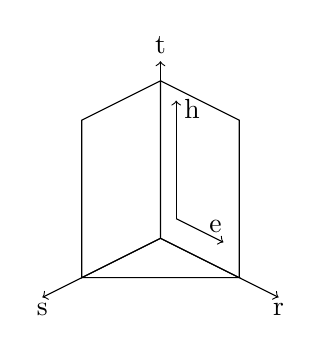
\begin{tikzpicture}
  \draw (0,-2) -- (1,-1.5) -- (1,0.5) --(0,0) --cycle;
  \draw (1,-1.5) -- (2,-2) -- (0,-2);
  \draw (1,0.5) -- (2,0) -- (2,-2);
  \draw [->] (1,-1.5) -- (2.5,-2.25);
  \draw [->] (1,-1.5) -- (-0.5,-2.25);
  \draw [->] (1,-1.5) -- (1,0.75) ;
  \draw [->] (1.2,-1.25) -- (1.2,0.25);
  \draw [->] (1.2,-1.25) -- (1.8,-1.55);
  \draw (2.5,-2.40) node {r};
  \draw (-0.5,-2.40) node {s};
  \draw (1,0.95) node{t};
  \draw (1.4,0.15) node{h};
  \draw (1.7,-1.35) node{e};
\end{tikzpicture}
\newline
The differential area vector along a boundary face equipped with an edge-wise ($e$) and
height-wise ($h$) coordinate system is given by :
\begin{equation}
  \vec{\partial s} = (\hat{e} \times \hat{h}) de dh
\end{equation}
The vectors $\hat{e}$ and $\hat{h}$ need to be expressed in the physical coordinate
system to reconstruct the expression for the differential area vector
in reference coordinates. Using the derivatives w.r.t $(h,e)$ as directional changes these
vectors can be expressed as:
\begin{eqnarray}
  \hat{e} = \frac{\partial x}{\partial e} \hat{e_x} + \frac{\partial y}{\partial e} \hat{e_y} + \frac{\partial z}{\partial e} \hat{e_z} \\
  \hat{h} = \frac{\partial x}{\partial h} \hat{e_x} + \frac{\partial y}{\partial h} \hat{e_y} + \frac{\partial z}{\partial h} \hat{e_z}
  \label{eq10}
\end{eqnarray}
The vectors $\hat{e}$ and $\hat{h}$ cannot however be arbitrary, they have to be constrained to
lie on the physical face of the element. This constraint can be also enforced by making sure they
lie on the planar face of the reference element. Each of the terms in Eq.~\ref{eq10},
$\frac{\partial x}{\partial e},\frac{\partial y}{\partial e},\frac{\partial z}{\partial e}..$ etc can be expanded as follows in terms of the
reference coordinates as
\begin{eqnarray}
  \frac{\partial x}{\partial e}=\frac{\partial x}{\partial r}\frac{\partial r}{\partial e} + \frac{\partial x}{\partial s}\frac{\partial s}{\partial e} + \frac{\partial x}{dt}\frac{dt}{\partial e} \\
  \frac{\partial y}{\partial e}=\frac{\partial y}{\partial r}\frac{\partial r}{\partial e} + \frac{\partial y}{\partial s}\frac{\partial s}{\partial e} + \frac{\partial y}{dt}\frac{dt}{\partial e} \\
  \frac{\partial z}{\partial e}=\frac{\partial z}{\partial r}\frac{\partial r}{\partial e} + \frac{\partial z}{\partial s}\frac{\partial s}{\partial e} + \frac{\partial z}{dt}\frac{dt}{\partial e} 
\end{eqnarray}
The equation for $\hat{h}$ is analogous. On inspection it follows that
\begin{eqnarray}
  \hat{e} =
  \begin{bmatrix}
  \frac{\partial x}{\partial r} & \frac{\partial x}{\partial s} & \frac{\partial x}{\partial t}\\
  \frac{\partial y}{\partial r} & \frac{\partial y}{\partial s} & \frac{\partial y}{\partial t}\\
  \frac{\partial z}{\partial r} & \frac{\partial z}{\partial s} & \frac{\partial z}{dt}
  \end{bmatrix}
  \begin{bmatrix}
    \frac{\partial r}{\partial e} \\
    \frac{\partial s}{\partial e} \\
    \frac{dt}{\partial e} \\
  \end{bmatrix}
  = J
  \begin{bmatrix}
    \frac{\partial r}{\partial e}\\
    \frac{\partial s}{\partial e}\\
    \frac{dt}{\partial e}\\
  \end{bmatrix} \\
    \hat{h} =
  \begin{bmatrix}
  \frac{\partial x}{\partial r} & \frac{\partial x}{\partial s} & \frac{\partial x}{\partial t}\\
  \frac{\partial y}{\partial r} & \frac{\partial y}{\partial s} & \frac{\partial y}{\partial t}\\
  \frac{\partial z}{\partial r} & \frac{\partial z}{\partial s} & \frac{\partial z}{\partial t}
  \end{bmatrix}
  \begin{bmatrix}
    \frac{\partial r}{\partial h} \\
    \frac{\partial s}{\partial h} \\
    \frac{dt}{\partial h} \\
  \end{bmatrix}
  = J
  \begin{bmatrix}
    \frac{\partial r}{\partial h}\\
    \frac{\partial s}{\partial h}\\
    \frac{dt}{\partial h}\\
  \end{bmatrix}
\end{eqnarray}

The vectors $a=\left[\frac{\partial r}{\partial e}, \frac{\partial s}{\partial e}, \frac{dt}{\partial e}\right]^T$ and
$b=\left[\frac{\partial r}{\partial h}, \frac{\partial s}{\partial h}, \frac{dt}{\partial h}\right]^T$ represent the constraint of being on the
boundary face and can be found trivially by following the variation of $(r,s,t)$ on the
respective  face of the reference element. For example,
$a=[1,0,0]$ and $b=[0,0,1]$ for the prismatic reference element shown earlier. The
differential area vector can now be expressed in the face coordinate system as:
\begin{equation}
  \vec{\partial s} = (\hat{e} \times \hat{h}) de dh
  = (Ja \times Jb) dedh
  \label{eq12}
\end{equation}
In 2-D, the $\hat{h}$ is just equal $\hat{e_z}$. So the elemental area (really arc length) reduces to
\begin{equation}
  \vec{\partial s} = (Ja \times \hat{e_z}) de 
\end{equation}
For a unit reference triangle, with coordinates $(0,0),(1,0),(0,1)$, the vector $a=[\frac{\partial r}{\partial e} \frac{\partial s}{\partial e}]^T$ is equal
to $[1,0]$, $[-1,1]$ and $[0,-1]$ for edges 1, 2 and 3 respectively. Several references (e.g. Ref~\cite{atkins}), at least to
my understanding, rewrite the tranformation of a differential area to the reference element as $J\vec{n_b} dedh$, where
$\vec{n_b}$ is the area scaled normal of the reference element face. Note that $\vec{n_b}$ is just $\vec{a} \times \vec{b}$.
To obtain this result from Eq.~\ref{eq12}, however $J$ must be a rotation matrix such that it satisfies $J^{-1}=J^T$. 
\subsection{Gradient Evaluation}
Gradient terms such as $\nabla b$, $\nabla q$ can be evaluated in the reference coordinates $\Lambda$,
by using the analytical derivatives of the basis functions, i.e.
\begin{eqnarray}
  (\nabla b)_\Lambda = \left[\frac{\partial b}{\partial r},\frac{\partial b}{\partial s},\frac{\partial b}{\partial t}\right]\\
  (\nabla Q)_\Lambda = \sum_{k=1}^{k=N} q_k(\nabla b_k)_\Lambda
\end{eqnarray}
The gradient in physical coordinates can be expressed by tranformation of coordinates as:
\begin{equation}
  (\nabla b) =
  \left[\frac{\partial b}{\partial r},\frac{\partial b}{\partial s},\frac{\partial b}{\partial t}\right]
  \begin{bmatrix}
  \frac{\partial r}{\partial x} & \frac{\partial r}{\partial y} & \frac{\partial r}{\partial z} \\
  \frac{\partial s}{\partial x} & \frac{\partial s}{\partial y} & \frac{\partial s}{\partial z} \\
  \frac{\partial t}{\partial x} & \frac{\partial t}{\partial y} & \frac{dt}{\partial z}
  \end{bmatrix}
  =(\nabla b)_\Lambda J^{-1}
\end{equation}

\subsection{Semi-discrete equation in reference coordinates}
Equation~\ref{eq8} can be now expressed in the reference element coordinates as:
\begin{equation}
  \left[\int_{\Lambda} {b_j} {b_k} |J| d\Lambda\right]\frac{\partial {(q_k)}_f}{\partial t} - \\
  \int_{\Lambda} \nabla b_j J^{-1}
  \cdot F(Q)_f |J| d \Lambda + \int_{\partial\Lambda} b_j F(Q)_f \cdot (J a \times J b) d\lambda  = 0
\label{eq13}
\end{equation}
Here $\Lambda$ and $d\Lambda$ are always within and around the reference element, i.e. their integration limits
are always $[0,1]$. The Jacobian $J\equiv J_i$ provides the scaling and rotation that maps the
physical element to the reference element.
Equation~\ref{eq13} can be further sub-divided as :
\begin{eqnarray}
  mass\_matrix=\left[M\right]=\left[\int_{\Lambda} {b_j} {b_k} |J| d\Lambda\right] \\
  volIntegral = \int_{\Lambda} \nabla b_j J^{-1}\cdot F(Q)_f |J| d \Lambda  \\
  faceIntegral = \int_{\partial\Lambda} b_j F(Q)_f \cdot (J a \times J b) d\lambda\\
  \left[M\right]\frac{\partial {(q_k)}_f}{\partial t} = volIntegral - faceIntegral
\end{eqnarray}
Once the right hand side of the above equation is evaluated, one can easily integrate in time using an explicit
Runge-Kutta type method. Implicit time stepping methods require linearization of the right hand side and will be
dealt with later.  Analytical evaluation of the integrals on the RHS is possible if all of the integrands can be expanded as
polynomial terms in $(r,s,t)$. A quadrature free approach~\cite{atkins} seeks to do exactly that. However, the
process of analytically determining all of the coefficients quickly becomes complicated for non-linear flux functions and
curved elements -- expansions of both fluxes and Jacobians has to computed as functions of polynomial coefficients. This
approach is not attempted at this point, although it is in the realm of possibilities to improve efficiency.
Currently standard quadrature based integration techniques, where each integral is found as a summation is used.
\subsection{Face Integral and connection between elements}
The defining feature of the DG method is the discontinuity of the solution field at element interfaces. So $F(Q)$ at the interface
is really a function of the states $Q_L$ and $Q_R$ or $\hat{F(Q)}.\vec{n} = \hat{F}(Q_L,Q_R,\vec(n))$. Therefore, the face
integral in the equations above has to be reconciled using a numerical flux function. The simplest approach for purely
convective flux is to use an upwind biased flux that can be expressed as:
\begin{equation}
  F(Q_L,Q_R).\vec{n} = \frac{1}{2}((F(Q_L)+F(Q_R).{\vec{n}} - \alpha (Q_R - Q_L) \vert\vert n \vert \vert)
\end{equation} 
Flux function based on Roe's approximate Riemann Solver~\cite{Roe}, which takes similar form as the equation above
is implemented. Any other flux function that can accept a left state, right state and a scaled normal vector as
arguments and output the numerical flux can be used. Note that for gradient dependent (diffusive type) fluxes, penalty
functions or lift operators need to be implemented to reconcile the discontinuity of derivatives at the element interfaces.
These will be implemented shortly.
\subsection{Quadrature rules}
All volume integrals, whose integrands can be represented as $I(r,s,t)$ are evaluated as
\begin{equation}
  \int_\Lambda I(r,s,t) d\Lambda = \sum_{g=1}^{g=M_g} w_g I(r_g,s_g,t_g)
\end{equation}
All face integrals, whose integrands can be represented as $J(r,s,t)$ are evaluated as
\begin{equation}
  \int_{d\Lambda} J(r,s,t) d \lambda = \sum_{g=1}^{g=M_f} w_g J(r(e_g,h_g),s(e_g,h_g),t(e_g,h_g))
\end{equation}
Where $(r_g,s_g,t_g,w_g)$ and $(e_g,h_g,w_g)$ are the locations and weights of the Gauss quadrature points for volume
and face integration respectively.

\section{Code architecture}
All data is stored in linear double precision arrays that can be indexed into using for each element. The integer array
$iptr$ provides the index into all volume data (geometry and solution), while the $iptf$ is the index list for all face data. The overall code execution follows the following pattern:
\begin{algorithm}
  \caption{\texttt{DGSAND}}
  \begin{algorithmic}[1]
    \State Read\_Grids()
    \State Find\_Connectivity()
    \State Allocate\_Memory()
    \State Initialize\_Grid\_And\_Solution\_Coefficients()
    \State Procedure{Compute\_Geometric\_Parameters()}
    \For {n=1:nsteps} 
     \For {r=1:rksteps} 
     \State $R_r \gets$ ComputeRHS($q_r,..$)
     \EndFor
     \State $q_{n+1} \gets$ update($q_n$,$R_1$,$R_2$..)
   \EndFor
  \end{algorithmic}
\end{algorithm}
Computing the right hand side is the most expensive operation. It is performed in 3 steps. First
all cells go through all of their bounding faces and project the solution to the face quadrature
points. Each face quadrature point has $3\times nfields$ storage space.
The face data is filled according a pre-deterimined fill order such that the cell on
the left side of the face fills $[0:nfields-1]$, the cell on the right side fills $[nfields:2*nfields-1]$, the last $nfields$ data space is left for the flux function to fill in the flux.
It is important to make sure that the face quadrature points are filled in the right order.
In 2-D this is easier to achieve with the left cell filling in forward order and right cell
filling in backward order. Arguably this is going to be one of the more complex topological
issues to solve in 3D. Once all the states on the left and right side are filled, each face
computes the Riemann flux using this states. At this point, each element has the full information
to completely compute the residual for all of its degrees of freedom and every element performs
this task. The execution follows a compute-scatter-compute-gather-compute, which avoids any
kind of race condition and can easily be multi-threaded. The algorithm is summarized below.
\begin{algorithm}
  \caption{\texttt{ComputeRHS}}
  \begin{algorithmic}[1]
    \For {i=1,$N_e$} \Comment{For each element}
    \For {f=1,$Nf_i$} \Comment{For each face of this element}
    \State FILL\_FACES() \Comment{fill states in to the face data array}
    \EndFor
    \EndFor
    \For {f=1,$Nbf$} \Comment{For each physical boundary face}
    \State FILL\_BC() \Comment{fill appropriate boundary condition states}
    \EndFor
    \For {f=1,$Nf$} \Comment{For all faces}
    \State COMPUTE\_FACE\_FLUXES() \Comment{find numerical flux on each face}
    \EndFor
    \For {i=1,$N_e$}
    \State $R_v \gets$ volumeIntegral() \Comment{volume integral using $M_g$ quadrature points}
    \For {f=1,$Nf_i$}
    \State $R_f \gets$ faceIntegral() \Comment{face integral using $M_f$ quadrature points}
    \EndFor
    \State $Residual \gets$ $R_v-R_f$
    \EndFor
  \end{algorithmic}
\end{algorithm}
%\section{Summary}
%This development guide is rough and unrefined and will be updated further as and when time
%allows for it.
\end{document}
